\documentclass[10pt]{scrartcl}
\usepackage[english]{babel}
\usepackage{multirow}
\usepackage[default]{opensans}
\usepackage{sfmath} % sans font also for math
\usepackage[binary-units = true]{siunitx}
\usepackage{graphicx}
% defining the paper layout that no text overlaps with the header
\usepackage[
  top=35mm,
  headheight=25mm,
  headsep=3mm,
  bottom=30mm,
  left=25mm,
  right=25mm
]{geometry}

\usepackage[verbose]{placeins}
\usepackage{subcaption}
\usepackage{latexsym}
\usepackage[centertags]{amsmath}
\usepackage{amssymb}
\usepackage[]{glossaries}

\graphicspath{{figures/}}
% custom header and footpage
\usepackage{scrpage2}
\pagestyle{scrheadings} % you have to set the custom layout
% Head
%\chead{}
\ohead{
\includegraphics[height=25mm]{figures/EUCALL.png}}
% Foot
\ifoot{
\includegraphics[height=13.4mm]{figures/EU.png}} % left foot
\cfoot{%
  \begin{minipage}{100mm}%
    \begin{scriptsize}%
      \normalfont{This project has received funding from the}
      \textit{European Union’s Horizon 2020 research and innovation programme}
      \normalfont{under grant agreement No 654220.}
    \end{scriptsize}%
  \end{minipage}%
} % center foot
\ofoot{\thepage} % right foot

\usepackage{booktabs}

%%%%%%%%%%%%%%%%%%%%%%%%%%%%%%%%%%%%%%%%%%%%%%%
%   BIBLIOGRAPHY SETTINGS
\usepackage[bibstyle=nature,sorting=none,maxnames=1000,eprint=false,
defernumbers=true, backend=biber]{biblatex}
\usepackage{chemformula}
\usepackage{hyperref}


\renewcommand*\finalnamedelim{, and\addspace}
\DeclareNameAlias{sortname}{last-first}
\renewcommand{\newunitpunct}{, }

\AtEveryBibitem{%
  \clearfield{day}%
  \clearfield{month}%
  \clearfield{endday}%
  \clearfield{endmonth}%
  \clearfield{issn}%
  \clearfield{issue}%
}
%convert titles to hyperlinks using doi
\ExecuteBibliographyOptions{doi=true} \newbibmacro{string+doi}[1]{%
  \iffieldundef{doi}{#1}{\href{http://dx.doi.org/\thefield{doi}}{#1}}}
  \DeclareFieldFormat*{title}{\usebibmacro{string+doi}{\mkbibemph{#1}}}

\addbibresource{urls.bib}
\addbibresource{footnotes.bib}
\addbibresource{library.bib}

%%%%%%%%%%%%%%%%%%%%%%%%%%%%%%%%%%%%%%%%%%%%%%%
% GLOSSARY SETTINGS
\setacronymstyle{long-short}
\input{glossary}
\makeglossaries
%%%%%%%%%%%%%%%%%%%%%%%%%%%%%%%%%%%%%%%%%%%%%%%

% Zeilenabstand
\renewcommand{\baselinestretch}{1.2}

\ihead{M4.3} % left head

% sophisticated linking of references in the pdf and setting some options
\usepackage{url}                                                  % for correct typesettings of URLs
\usepackage{hyperref}                                             % for sophisticated linking of urls, dois, pictures, tables, etc.
\hypersetup{
    unicode=true,                                                 % non-Latin characters in Acrobat’s bookmarks
    pdftoolbar=true,                                              % show Acrobat’s toolbar?
    pdfmenubar=true,                                              % show Acrobat’s menu?
    pdffitwindow=false,                                           % window fit to page when opened
    pdfstartview={FitH},                                          % fits the width of the page to the window
    pdftitle={M4.3: Interoperable simulations},                                        % title
    pdfauthor={C. Fortmann-Grote},                                           % author
    pdfsubject={EUCALL WP4 (SIMEX) Deliverable D4.3},                             % subject of the document
    pdfcreator={pdflatex},                                         % creator of the document
    pdfkeywords={EUCALL, SIMEX, simulations, Rad-Hydro, XFEL, ESRF, warm dense
    matter, absorption, radiography},                                         % list of keywords
    pdfnewwindow=true,                                            % links in new PDF window
    colorlinks=true,                                              % false: boxed links; true: colored links
    linkcolor=blue,                                                % color of internal links (change box color with linkbordercolor)
    citecolor=blue,                                                % color of links to bibliography
    filecolor=blue,                                               % color of file links
    urlcolor=blue                                                 % color of external links
}

\begin{document}
\makeatletter
\begin{titlepage}
\thispagestyle{scrheadings}
\begin{center}
  $~$\\
  \vspace{2cm}
  \Huge{\textbf{WP 4 -- SIMEX\\[1cm]
    Milestone M4.3: Simulations interoperable%
  }}\\
  \vspace{2cm}
  \large{%
    Carsten Fortmann-Grote
  }\\[1cm]
  \today
\end{center}
\vfill%
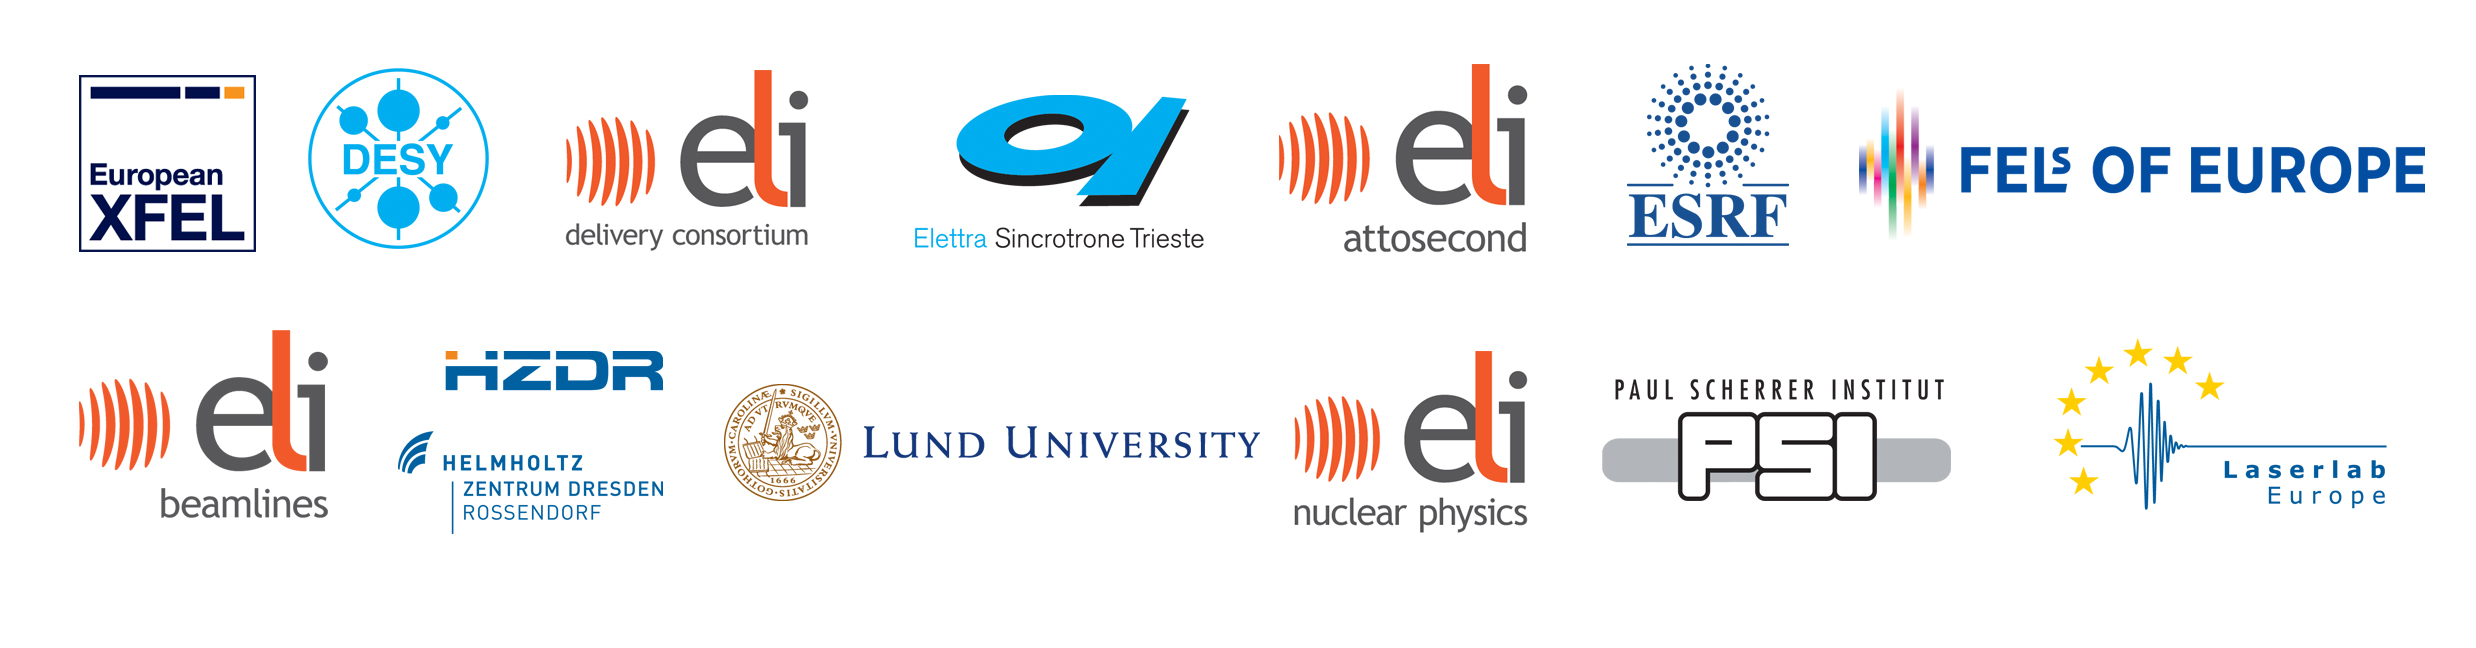
\includegraphics[width=\textwidth]{figures/PartnerLogos_2017}
\end{titlepage}
\makeatother

%\tableofcontents

\section{Summary}
%
Simulations in SIMEX are now interoperable. The simulation platform
\textit{simex\_platform}
\cite{Fortmann-Grote2016b,Fortmann-Grote2017a,simex_github}, publicly available from \href{https://www.github.com/eucall-software/simex_platform}{https://www.github.com/eucall-software/simex\_platform} under the conditions of the open source license GPL-v3 \cite{gplv3}, enables start--to--end simulations of various types of photon experiments using
different sources (X--ray free electron lasers, synchrotrons, optical lasers),
different means of photon propagation from the source to the sample (coherent
wavefront propagation, x--ray tracing), various types of photon matter
interaction (particle--in--cell, radiation--hydrodynamics, molecular dynamics,
continuum plasma theory), signal generation (coherent diffraction from plasma
and non--plasma samples, inelastic scattering, x--ray absorption spectroscopy)
and detector simulations.

Details and use cases, demonstrating how the various
simulation modules can be used in an interoperable and interchangeable way are
given in the Milestone document M4.2 \cite{EUCALL_SIMEX_M4.2} and Deliverable
Report D4.3~\cite{EUCALL_SIMEX_D4.3}. In particular, use of custom as well as generic
metadata standards and data formats facilitate the transfer of simulation data
between modules, which fulfills the requirement of ``interoperability''.

Modules are interchangeable, e.g. a coherent diffraction
imaging experiment for a molecular sample can be altered into a diffraction
experiment for a crystalline sample by switching just one
simulation module, the signal generator.
These and other applications are also demonstrated in online tutorials, located
on the wiki pages of \textit{simex\_platform} at
\href{https://www.github.com/eucall-software/simex_platform/wiki}{https://www.github.com/eucall-software/simex\_platform/wiki}.

The release of version 0.3.3 of \textit{simex\_platform} \cite{simex0.3.3} marks
the project milestone M4.3.

\printbibliography
%%%%%%%%%%%%%%%%%%%%%%%%%%%
\end{document}


